%==============================================================================
\chapter{Scalable RDF querying}
\label{chapter:scalable_rdf_querying}
%==============================================================================
In the recent years, our information society has reached the stage where it produces billions of data records, amounting to multiple quintillion of bytes\furl{https://www.domo.com/learn/data-never-sleeps-5}, on a daily basis.
Extraction, cleansing, enrichment and refinement of information are key to fuel value-adding processes, such as analytics as a premise for decision making.
Devising appropriate (ideally uniform) representations and facilitating efficient querying of data, metadata and provenance arising from such phases constantly poses challenges, especially when data volumes are vast.
The most prominent and promising effort is the \gls{W3C} consortium with encouraging \gls{RDF} as a common data representation and vocabularies (e.g. RDFS, \gls{OWL}) as a way to include meta-information about the data.
These data and meta-data can be further processed and analyzed using the de-facto query language for \gls{RDF} data, \gls{SPARQL}.
\gls{SPARQL} serves as a standard query language for manipulating and retrieving \gls{RDF} data.

Querying \gls{RDF} data becomes challenging when the size of the data increases. 
This has motivated a considerable amount of work on designing distributed \gls{RDF} systems able to efficiently evaluate \gls{SPARQL} queries (\cite{Schatzle:2016:SRQ:2977797.2977806,sparqlgx-iswc-2016}).
Being able to query a large amount of data in an efficient and faster way is one of the key requirements for every \gls{SPARQL} engine.

To address these challenges, in this thesis, we propose a scalable \gls{RDF} querying engine based on two different partitioning strategies.
First, Sparklify -- SPARQL-to-SQL rewriter based on the vertical partitioning implemented on top of Apache Spark.
As a second approach, we investigated and developed the so-called Semantic-based query system. 
Both approaches are a scalable and efficient evaluation of \gls{SPARQL} queries over distributed \gls{RDF} datasets. 
The main component of the both systems are the data partitioning and query evaluation over this data representation.

In this chapter we address the following research question:
\begin{tcolorbox}
\textbf{RQ3}: Can distributed \gls{RDF} datasets be queried efficiently and effectively?
\end{tcolorbox}

Contributions of this chapter are summarized as follows:

\begin{itemize}
 \item We present a novel approach for vertical partitioning including \gls{RDF} terms using the distributed computing framework, Apache Spark.
 \item We developed a scalable query system using Sparqlify -- a SPARQL-to-SQL rewriter on top of Apache Spark (under the \textit{Apache Licence 2.0}).
 \item We evaluate Sparklify with state-of-the-art engines and demonstrate it empirically.
 \item A scalable approach for semantic-based partitioning using the distributed computing framework, Apache Spark.
 \item A scalable semantic-based query engine (\textit{SANSA.Semantic}) on top of Apache Spark.
 \item Comparison of the semantic-based system with state-of-the-art engines and demonstrate the performance empirically.
 \item We integrated the proposed approaches into the SANSA~\cite{lehmann-2017-sansa-iswc}\furl{http://sansa-stack.net/} larger framework.
 Sparklify serves as a default query engine in SANSA.
 SANSA is an active project and maintained, including issue tracker, mailing list, changelogs, website, etc.
\end{itemize}


This chapter is based on the following publications (\cite{sejdiu-2019-sansa-semantic-based-semantics,2019-sansa-sparklify-iswc, sansa-sparklify-ISWC-demo}):
\begin{itemize}
     \item \textbf{Gezim Sejdiu}; Damien Graux; Imran Khan; Ioanna Lytra; Hajira Jabeen; and Jens Lehmann, “\href{https://gezimsejdiu.github.io/publications/semantic_based_query_paper_SEMANTICS2019.pdf}{Towards A Scalable Semantic-based Distributed Approach for SPARQL query evaluation},” 15th International Conference on Semantic Systems (SEMANTiCS), Research \& Innovation , 2019.
     
    \item Claus Stadler; \textbf{Gezim Sejdiu}; Damien Graux; and Jens Lehmann, “\href{http://jens-lehmann.org/files/2019/iswc_sparklify.pdf}{Sparklify: A Scalable Software Component for Efficient evaluation of SPARQL queries over distributed RDF datasets},” in Proceedings of 18th International Semantic Web Conference (ISWC), 2019. 
    This article is a joint work with Claus Stadler, a PhD student at the University of Leipzig. 
    In this article, I devised the implementation of the conceptual architecture, helped on the implementation of the proposed approach, reviewed related work, and prepared of the experiments and analysis of the obtained results.
    
    \item Claus Stadler; \textbf{Gezim Sejdiu}; Damien Graux; and Jens Lehmann. "\href{https://gezimsejdiu.github.io/publications/sansa-sparklify-ISWC-demo.pdf}{Querying large-scale RDF datasets using the SANSA framework}".  In Proceedings of 18th International Semantic Web Conference (ISWC), Poster \& Demos, 2019.
\end{itemize}

The rest of the chapter is structured as follows:
Sparklify, a scalable software component for \gls{SPARQL} evaluation of large \gls{RDF} data is presented in Section~\ref{sec:sparklify-approach}.
Its data modeling, data partitioning, and query translation using a distributed framework (Apache Spark) are detailed in Subsection~\ref{sec:sparklify-architecture} and evaluated in Subsection~\ref{sec:sparklify-evaluation}.
Second part of the chapter, Suction~\ref{sec:semantic-based-approach} elaborate the Semantic-based approach, including its system architecture overview as presented in Section~\ref{fig:semantic-based-architecture}.
The Semantic-based approach is evaluated in Subsection~\ref{sec:semantic-based-evaluation}.
Finally, we summarize our work in  Section~\ref{sec:scalable-rdf-querying-summary}.

\section{Sparklify: Scalable Software for SPARQL evaluation of large RDF data}
\label{sec:sparklify-approach}
In this section, we present the overall architecture of Sparklify, the SPARQL-to-SQL rewriter, and mapping to Spark Scala-compliant code.

\subsection{System Architecture Overview}
\label{sec:sparklify-architecture}

The overall system architecture is shown in Figure~\ref{fig:sparklify-architecture}.
It consists of four main components: Data Model, Mappings, Query Translator and Query Evaluator.
In the following, each component is discussed in details.

\begin{figure*}
\centering
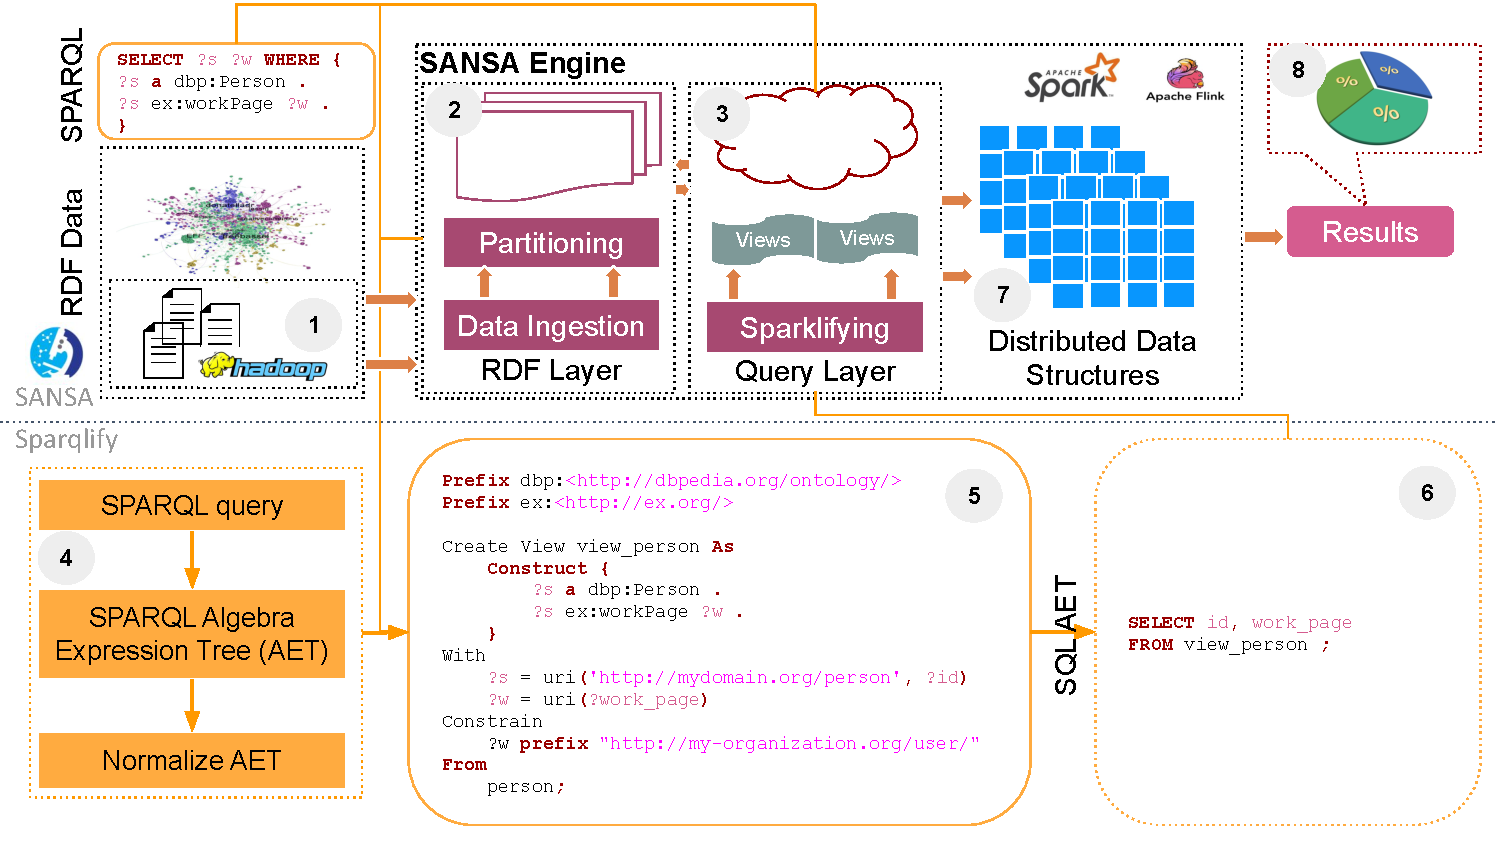
\includegraphics[width=1.0\textwidth]{images/6_scalable_rdf_querying/sparklify-architecture.pdf}
\caption{\textbf{Sparklify Architecture Overview}.
It consists of four main components: Data modeling -- data ingestion and data partitioning (using the extensible vertical paritioning), Mappings/Views -- the relational-to-RDF mapping, Query Translator -- SQL query generator from the SPARQL query, and Query Evaluator - SQL query evaluated directly into the Spark SQL engine.
}
% source : https://docs.google.com/presentation/d/16XlT4u3bFn8XdP_eoLJOAu5WPl_q_9zIjAZbllfEEic 
\label{fig:sparklify-architecture}
% source : 
\end{figure*}


\defn{Data Model}
SANSA~\cite{lehmann-2017-sansa-iswc} comes with different data structures and different partitioning strategies.
We model and store \gls{RDF} graph following the concept of \gls{RDD}s -- a basic building blocks of the Spark Framework.
\gls{RDD}s are in-memory collections of records which are capable of operating in parallel overall larger cluster.
Sparklify makes use of SANSA bottom layer which corresponds with the extended vertical partitioning (VP) including \gls{RDF} terms.
This partition model is the most convenient storage model for fast processing of \gls{RDF} datasets on top of \gls{HDFS}.
\paragraph{Data Ingestion (Step 1)} \gls{RDF} data first needs to be loaded into a large-scale storage that Spark can efficiently read from.
We use \gls{HDFS}.
Spark employ different data locality scheme in order to accomplish computations nearest to the desired data in \gls{HDFS}, as a result avoiding i/o overhead. 
\paragraph{Data Partition (Step 2)}
VP approach in SANSA is designed to support extensible partitioning of \gls{RDF} data.
Instead of dealing with a single three-column table $(s, p, o)$, data is partitioned into multiple tables based on the used \gls{RDF} predicates, \gls{RDF} term types and literal datatypes.
The first column of these tables is always a string representing the subject.
The second column always represents the literal value as a Scala/Java datatype.
Tables for storing literals with language tags have an additional third string column for the language tag.

\defn{Mappings/Views}
After the \gls{RDF} data has been partitioned using the extensible VP (as it has been described on \textit{Step 2}) the relational-to-RDF mapping is performed. 
Sparqlify supports both the \gls{W3C} standard R2RML
sparqlification~\cite{sml}.

The main entities defined with SML are \textit{view definitions}.
See \textit{Step 5} in the Figure~\ref{fig:sparklify-architecture} as an example.
The actual view definition is declared by the \emph{Create View} \ldots \emph{As} in the first line.
The remainder of the view contains these parts: (1) the \emph{From} directive defines the logical table based on the partitioned table (see \textit{Step 2}).
(2) an RDF template is defined in the \emph{Construct} block containing, \gls{URI}, blank node or literals constants (e.g. \emph{ex:worksAt}) and variables (e.g. \emph{?emp}, \emph{?institute}).
The \emph{With} block defines the variables used in the template by means of \gls{RDF} term constructor expressions whose arguments refer to columns of the logical table.

\defn{Query Translation}
This process generates a SQL query from the \gls{SPARQL} query using the bindings determined in the mapping/view construction phases.
It walks through the \gls{SPARQL} query (\textit{Step 4}) using Jena ARQ\furl{https://jena.apache.org/documentation/query/} and generates the \gls{SPARQL} \gls{AET}. 
Essentially, rewriting \gls{SPARQL} basic graph patterns and filters over views yields \gls{AET}s that are UNIONS of JOINS.
Further, these AETs are normalized and pruned in order to remove UNION members that are known to yield empty results, such as joins based on \gls{IRI}s with disjoint sets of known namespaces, or joins between different \gls{RDF} term types (e.g. literal and \gls{IRI}).
Finally, the SQL is generated (\textit{Step 6}) using the bindings corresponding to the views (\textit{Step 5}).

\defn{Query Evaluator}
The SQL query created as described in the previous section can now be evaluated directly into the Spark SQL engine.
The result set of this SQL query is distributed data structure of Spark (e.g. DataFrame) (\textit{Step 7}) which then is mapped into a \gls{SPARQL} bindings.
The result set can further used for analysis and visualization using the SANSA-Notebooks (\textit{Step 8})~\cite{iermilov-2017-sansa-iswc-demo}.


\subsection{Evaluation}
\label{sec:sparklify-evaluation}

The goal of our evaluation is to observe the impact of the extensible VP as well as analyzing its scalability when the size of the dataset increases.
At the same time, we also want to measure the effect of using Sparqlify optimizer for improving the query performance.
Especially, we want to verify and answer the following questions:
\begin{itemize}
\addtolength{\itemindent}{1cm}
    \newitem[Q1]\label{item:Q1}: Is the runtime affected when more nodes are added in the cluster?
    \newitem[Q2]\label{item:Q2}: Does it scale to a larger dataset?
    \newitem[Q3]\label{item:Q3}: How does it scale when adding a larger number of datasets?
\end{itemize}
In the following, we present our experiments setting including the benchmarks used and server configurations. 
Afterword, we elaborate on our findings.

\subsubsection{Experimental Setup}
We used two well-known \gls{SPARQL} benchmarks for our evaluation. 
The \textit{Lehight University Benchmak (LUBM)} v3.1~\cite{Guo2005LUBMAB} and \textit{Waterloo SPARQL Diversity Test Suite (WatDiv)} v0.6~\cite{Alu2014DiversifiedST}.
Characteristics of the considered datasets are given in Table~\ref{tab:sparklify-dataset_info}.

\textit{LUBM} comes with a \textit{Data Generator (UBA)} which generates synthetic data over the \textit{Univ-Bench} ontology in the unit of a university.
Our \textit{LUBM} datasets consist of 1000, 5000, and 10000 universities.
The number of triples varies from 138M for 1000 universities, to 1.4B triples for 10000 universities.
\textit{LUBM}'s test suite is comprised of 14 queries.

We have used \textit{WatDiv} datasets with approximate 10K to 1B triples with scale factors 10, 100 and 1000, respectively. 
\textit{WatDiv} provides a test suite with different query shapes, therefore, it allows us to compare the performance of Sparklify and the other approach we compare with in a more compact way.
We have generated these queries using the \textit{WatDiv Query Generator} and report the average mean runtime in the overall results presented below.
It comes with a set of 20 predefined query templates so-called \textit{Basic Testing Use Case} which is grouped into four categories, based on the query shape : \textit{star (QS)}, \textit{linear (QL)}, \textit{snowflake (QF)}, and \textit{complex (QC)}.

\begin{table*}
\centering
\begin{tabularx}{\textwidth}{Xccccccc}	
\toprule
\multirow{2}{*}{$\longrightarrow$} & \multicolumn{3}{c|}{LUBM} & \multicolumn{4}{c}{Watdiv} \\
\cline{2-8}  \rule{0pt}{10pt}
&   \scriptsize{1K} & \scriptsize{5K} & \scriptsize{10K}  & \scriptsize{10M} &\scriptsize{100M} &\scriptsize{1B} &\\
\midrule
\scriptsize{\#nr. of triples}& \scriptsize{138,280,374} & \scriptsize{690,895,862} & \scriptsize{1,381,692,508} & \scriptsize{10,916,457} & \scriptsize{108,997,714} & \scriptsize{1,099,208,068} &  \\
\scriptsize{size (GB)}  & \scriptsize{24} & \scriptsize{116} & \scriptsize{232} & \scriptsize{1.5} &\scriptsize{15} &\scriptsize{149} &\\
\bottomrule
\end{tabularx}
{\caption{\textbf{Summary information of used datasets (nt format)}.
Lists dataset characteristics used on the evaluation.
The size (in GB) and the number of triples are given.}
\label{tab:sparklify-dataset_info}}
\end{table*}

We implemented Sparklify using Spark-2.4.0, Scala 2.11.11, Java 8, and Sparqlify 0.8.3 and all the data were stored on the \gls{HDFS} cluster using Hadoop 2.8.0.
All experiments were carried out on a commodity cluster of 7 nodes (1 master, 6 workers): Intel(R) Xeon(R) CPU E5-2620 v4 @ 2.10GHz (32 Cores), 128 GB RAM, 12 TB SATA RAID-5, connected via a Gigabit network.
The experiments have been executed three times and the average runtime has been reported into the results.

\subsubsection{Results}
We evaluate Sparklify using the above datasets and compare it with the chosen state-of-the-art distributed \gls{SPARQL} query evaluator.
Since our approach does not involve any pre-processing of the RDF data before being able to evaluate \gls{SPARQL} queries on it, Sparklify is thereby closer to the so-called direct evaluators.
Indeed, Sparklify only needs to virtually partition the data prior.
As a consequence, we omit other distributed evaluators (such as e.g. S2RDF~\cite{Schatzle:2016:SRQ:2977797.2977806}) and compare it with SPARQGX~\cite{sparqlgx-iswc-2016} as it outperforms other approaches as noted by Graux et.al~\cite{sparqlgx-iswc-2016}.
We compare our approach with \emph{SPARQLGX}'s direct evaluator named SDE and report the loading time for partitioning and query execution time, see Table~\ref{tbl:sparklify-performance-analysis}.
We specify ``fail'' whenever the system fails to complete the task and ``n/a'' when the task could not be completed due to a failure in one of the intermediate phase.
In some cases e.g. in Table~\ref{tbl:sparklify-performance-analysis}, \textit{QC in Watdiv-1B} dataset, we define "partial fail" due to the failure of one of the queries, therefore the sum-up is not possible.

Findings of the experiments are depicted in Table~\ref{tbl:sparklify-performance-analysis}, Figure~\ref{fig:sparklify-sizeup-scalability}, \ref{fig:sparklify-node-scalability}, and  \ref{fig:sparklify-overall-analysis}.

To verify \ref{item:Q1}, we analyze the \textit{speedup} and compare it with SPARQLGX.
We run the experiments on three datasets, \emph{Watdiv-10M}, \emph{Watdiv-1B} and \emph{LUBM-10K}.

\begin{table*}[t]
\centering
\begin{tabularx}{\textwidth}{*{6}{X}}	
\toprule
\multicolumn{1}{l}{}& \multicolumn{4}{c}{\scriptsize{Runtime (s)} (\scriptsize{mean})} \\
\cline{2-5}
\rule{0pt}{8pt}
\multirow{2}{*}{$\longrightarrow$} & \multicolumn{1}{c|}{\scriptsize{\textbf{SPARQLGX-SDE}}} & \multicolumn{3}{c}{\scriptsize{\textbf{Sparklify}}} \\
\cline{2-5}  \rule{0pt}{10pt}
& \scriptsize{a) total} & \scriptsize{b) paritioning}  & \scriptsize{c) querying} & \scriptsize{d) total} \\
\midrule
\multirow{5}{*}{\rotatebox{90}{\scriptsize{\textbf{Watdiv-10M}}}}
&  & & & \\
\hspace{0.2cm} $QC$ & \win \scriptsize{103.24} & \scriptsize{134.81} & \win \scriptsize{61} & \scriptsize{195.84} \\
\hspace{0.2cm} $QF$ & \win \scriptsize{157.8} & \scriptsize{241.24} & \win \scriptsize{107.33} & \scriptsize{349.51}  \\
\hspace{0.2cm} $QL$ & \win \scriptsize{102.51} & \scriptsize{236.06} & \scriptsize{134} & \scriptsize{370.3} \\
\hspace{0.2cm} $QS$ & \win \scriptsize{131.16} & \scriptsize{237.12} & \win \scriptsize{108.56} & \scriptsize{346} \\
\midrule
\multirow{5}{*}{\rotatebox{90}{\scriptsize{\textbf{Watdiv-1B}}}}
&  & & &  \\
\hspace{0.2cm} $QC$ & \textcolor{red}{\scriptsize{partial fail} }& \win \scriptsize{778.62} & \win \scriptsize{2043.66} & \win \scriptsize{2829.56} \\
\hspace{0.2cm} $QF$ & \scriptsize{6734.68} & \win \scriptsize{1295.31} & \win \scriptsize{2576.52} & \win \scriptsize{3871.97} \\
\hspace{0.2cm} $QL$ & \scriptsize{2575.72} & \win \scriptsize{1275.22} & \win \scriptsize{610.66} & \win \scriptsize{1886.73} \\
\hspace{0.2cm} $QS$ & \scriptsize{4841.85} & \win \scriptsize{1290.72} & \win \scriptsize{1552.05} & \win \scriptsize{2845.3} \\
\midrule
\multirow{14}{*}{\rotatebox{90}{\scriptsize{\textbf{LUBM-10K}}}}
$Q1$ & \win \scriptsize{1056.83} & \scriptsize{627.72} & \scriptsize{718.11} & \scriptsize{1346.8}\\
\hspace{0.2cm} $Q2$ & \textcolor{red}{\scriptsize{fail}} & \scriptsize{595.76} & \textcolor{red}{\scriptsize{fail}} &  \scriptsize{n/a} \\
\hspace{0.2cm} $Q3$ & \win \scriptsize{1038.62} & \scriptsize{615.95} & \scriptsize{648.63} &  \scriptsize{1267.37} \\
\hspace{0.2cm} $Q4$ & \scriptsize{2761.11} & \win \scriptsize{632.93} & \win \scriptsize{1670.18} &  \win \scriptsize{2303.18} \\
\hspace{0.2cm} $Q5$ & \win \scriptsize{1026.94} & \scriptsize{641.53} & \scriptsize{564.13} &  \scriptsize{1206.67}\\
\hspace{0.2cm} $Q6$ & \win \scriptsize{537.65} & \scriptsize{695.74} & \scriptsize{267.48} &  \scriptsize{963.62}\\
\hspace{0.2cm} $Q7$ & \scriptsize{2080.67} & \win \scriptsize{630.44} & \win \scriptsize{1331.13} &  \win \scriptsize{1967.25}\\
\hspace{0.2cm} $Q8$ & \scriptsize{2636.12} & \win \scriptsize{639.93} & \win \scriptsize{1647.57} &  \win \scriptsize{2288.48} \\
\hspace{0.2cm} $Q9$ & \scriptsize{3124.52} & \win \scriptsize{583.86} & \win \scriptsize{2126.03} &  \win \scriptsize{2711.24} \\
\hspace{0.2cm} $Q10$ & \win \scriptsize{1002.56} & \scriptsize{593.68} & \scriptsize{693.73} &  \scriptsize{1287.71} \\
\hspace{0.2cm} $Q11$ & \win \scriptsize{1023.32} & \scriptsize{594.41} & \scriptsize{522.24} &  \scriptsize{1118.58}\\
\hspace{0.2cm} $Q12$ & \scriptsize{2027.59} & \win \scriptsize{576.31} & \win \scriptsize{1088.25} &  \win \scriptsize{1665.87} \\
\hspace{0.2cm} $Q13$ & \scriptsize{1007.39} & \win \scriptsize{626.57} & \win \scriptsize{6.66} &  \win \scriptsize{633.26} \\
\hspace{0.2cm} $Q14$ & \win \scriptsize{526.15} & \scriptsize{633.39} & \scriptsize{258.32} &  \scriptsize{891.89}\\
\bottomrule
\end{tabularx}
{\caption{\textbf{Performance analysis on large-scale RDF datasets}.
Comparison analysis of Sparklify as compared with \emph{SPARQLGX}'s direct evaluator named SDE.
The loading time for partitioning and query execution time is reported.
}
\label{tbl:sparklify-performance-analysis}}
\end{table*} %source : https://docs.google.com/spreadsheets/d/16CcsZcmrGF0yevu8L5mlAALGB2JZvHNkS4-6WQV0edo

Table~\ref{tbl:sparklify-performance-analysis} shows the performance analysis of two approaches run on three different datasets.
Column SPARQLGX-SDE$^{a}$ reports on the performance of SPARQLGX-SDE considering the total runtime to evaluate the given queries.
Column Sparklify$^{b}$ lists the times required for Sparklify to perform the VP and then the query execution time is reported on the Sparklify$^{c}$.
Total runtime for Sparklify is shown in the last column, Sparklify$^{d}$.

We observe that the execution of both approaches fails for the \textit{Q2} in the \textit{LUBM-10K} dataset while evaluating the query. 
We believe that it is due to the reason that \textit{LUBM Q2} involves a triangular pattern which is often resource consuming. 
As a consequence, in both cases, Spark performs the shuffling (e.g. data scanning) while reducing the result set.
It is interesting to note that for the \textit{Watdiv-1B} dataset, SPARQLGX-SDE fails for the query \textit{C3} when data scanning is performed. 
Sparklify is capable of evaluating it successfully.
Due to the Spark SQL optimizer in conjunction with Sparqlify's approach of rewriting a SPARQL query typically into only a single SQL query -- effectively offloading all query planning to Spark -- Sparklify performs better than SPARQLGX-SDE when the size of the dataset increases (see \textit{Watdiv-1B results} in the Table~\ref{tbl:sparklify-performance-analysis}) and when there are more joins involved (see \textit{Watdiv-1B} and \textit{LUBM-10K} results in the Table~\ref{tbl:sparklify-performance-analysis}).
SPARQLGX-SDE evaluates the queries faster when the size of the datasets is smaller, but it degrades when the size of the dataset increases.
The likely reason for Sparklify's worse performance on smaller datasets is its higher partitioning overhead.
Figure~\ref{fig:sparklify-sizeup-scalability} shows that Sparklify starts outperforming when the size of the datasets grows (e.g. \textit{Watdiv-100M}).

\defn{Size-up scalability analysis}
To measure the performance of the data scalability (e.g. size-up) of both approaches, we run experiments on three different sizes of \textit{Watdiv} (see Figure~\ref{fig:sparklify-sizeup-scalability}).

\begin{figure*}
 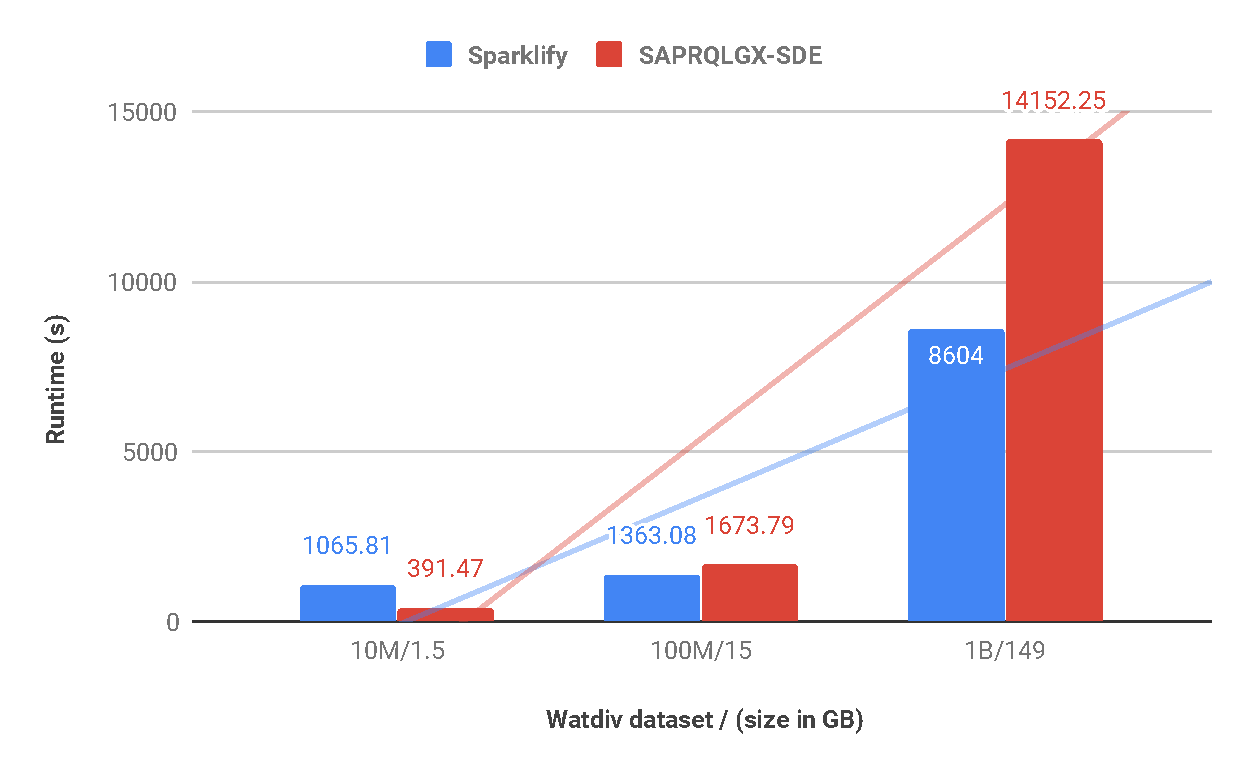
\includegraphics[width=1.0\columnwidth]{images/6_scalable_rdf_querying/sparklify-sizeup-scalability.pdf}
    \caption{\textbf{Sizeup analysis (on Watdiv dataset)}.
    The analysis keep the number of nodes constant i.e. 6 worker nodes and grow the size of the dataset (Watdiv) in order to measure whether the approaches chosen for evaluation can deal with larger datasets.
    As depicted, the execution time for Sparklify grows linearly as compared with SPARQLGX-SDE, and keep staying near-linear when the size of the dataset increases.}
    \label{fig:sparklify-sizeup-scalability}
\end{figure*}

We keep the number of nodes constant i.e 6 worker nodes and grow the size of the datasets to measure whether both approaches can deal with larger datasets.
We see that the execution time for Sparklify grows linearly compared with SPARQLGX-SDE, which keeps staying as near-linear when the size of the datasets increases. 
The results presented show scalability of Sparklify in context of the sizeup, which addresses the question \ref{item:Q2}.

\defn{Node scalability analysis}
To measure the node scalability of Sparklify, we vary the number of worker nodes.
We vary them from 1, 3 to 6 worker nodes.

\begin{figure*}
  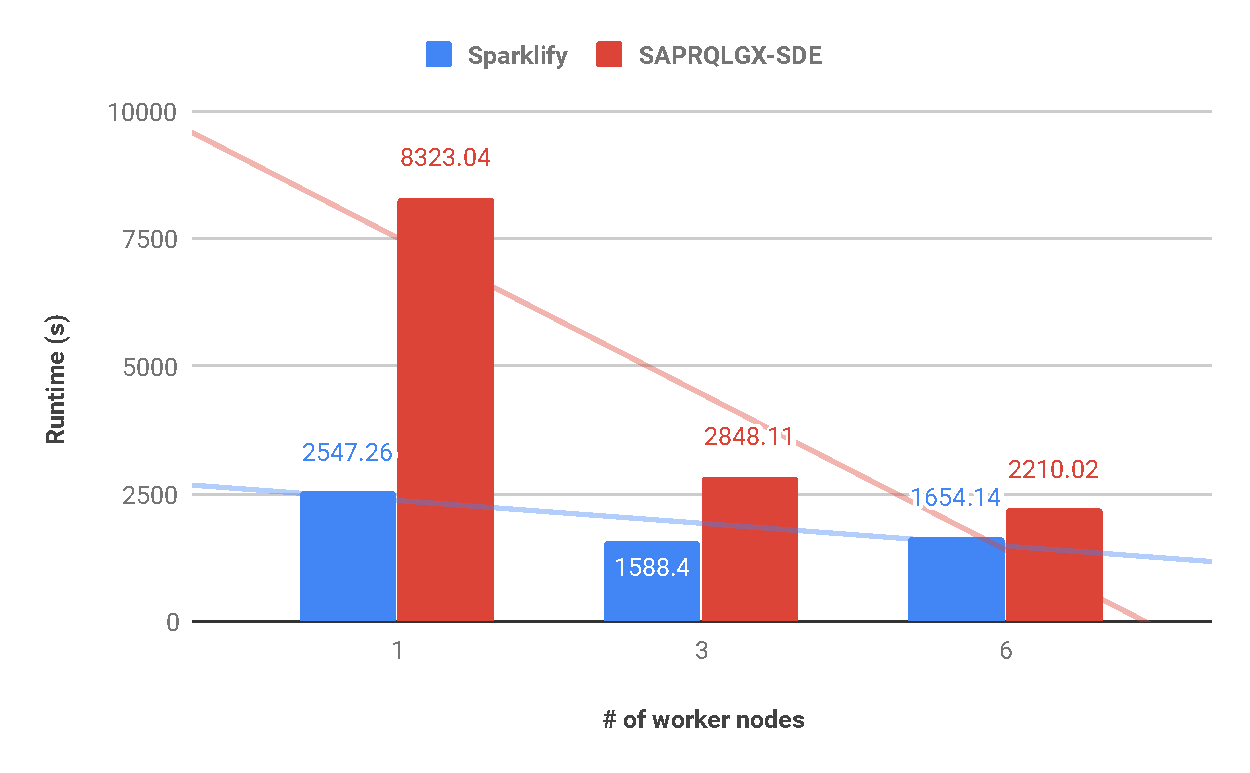
\includegraphics[width=1.0\columnwidth]{images/6_scalable_rdf_querying/sparklify-node-scalability.pdf}
    \caption{\textbf{Node scalability (on Watdiv-100M)}.
    The analysis vary the number of worker nodes e.g. from 1, 3, to 6 worker nodes and keep the size of the dataset constant i.e. \textit{Watdiv-100M}.
    It shows that as the number of nodes increases, the runtime cost for Sparklify decreases linearly.
    It decreases about 0.6 times (from 2547.26 seconds down to 1588.4 seconds) as worker nodes increase from one to three nodes.}
    \label{fig:sparklify-node-scalability}
\end{figure*}

Figure~\ref{fig:sparklify-node-scalability} depict the speedup performance of both approaches run on \textit{Watdiv-100M} datasaet when the number of worker nodes varies.
We can see that as the number of nodes increases, the runtime cost for the Sparklify decrease linearly.
The execution time for Sparklify decreases about 0.6 times (from 2547.26 seconds down to 1588.4 seconds) as worker nodes increase from one to three nodes.
We see that the speedup stays constant when more worker nodes are added since the size of the data is not that large and the network overhead increases a little the runtime when it runs over six worker nodes.
This imply that our approach is efficient up to three worker nodes for the \textit{Watdiv-100M} (15GB) dataset.
In another hand, SPARQLGX-SDE takes longer to evaluate the queries when running on one worker node but it improves when the number of worker nodes increases.

Result presented here shows that Sparklify can achieve linear scalability in the performance, which addresses \ref{item:Q3}.

\defn{Correctness of the result set}
In order to assess the correctness of the result set, we computed the count of the result set for the given queries and compare it within both approaches.
We conclude that both approaches return exactly the same result set which implies the correctness of the results.

\defn{Overall analysis by \gls{SPARQL} queries}
Here we analyze Watdiv queries run on \textit{Watdiv-100M} dataset in a cluster mode on both approaches.

\begin{figure}
  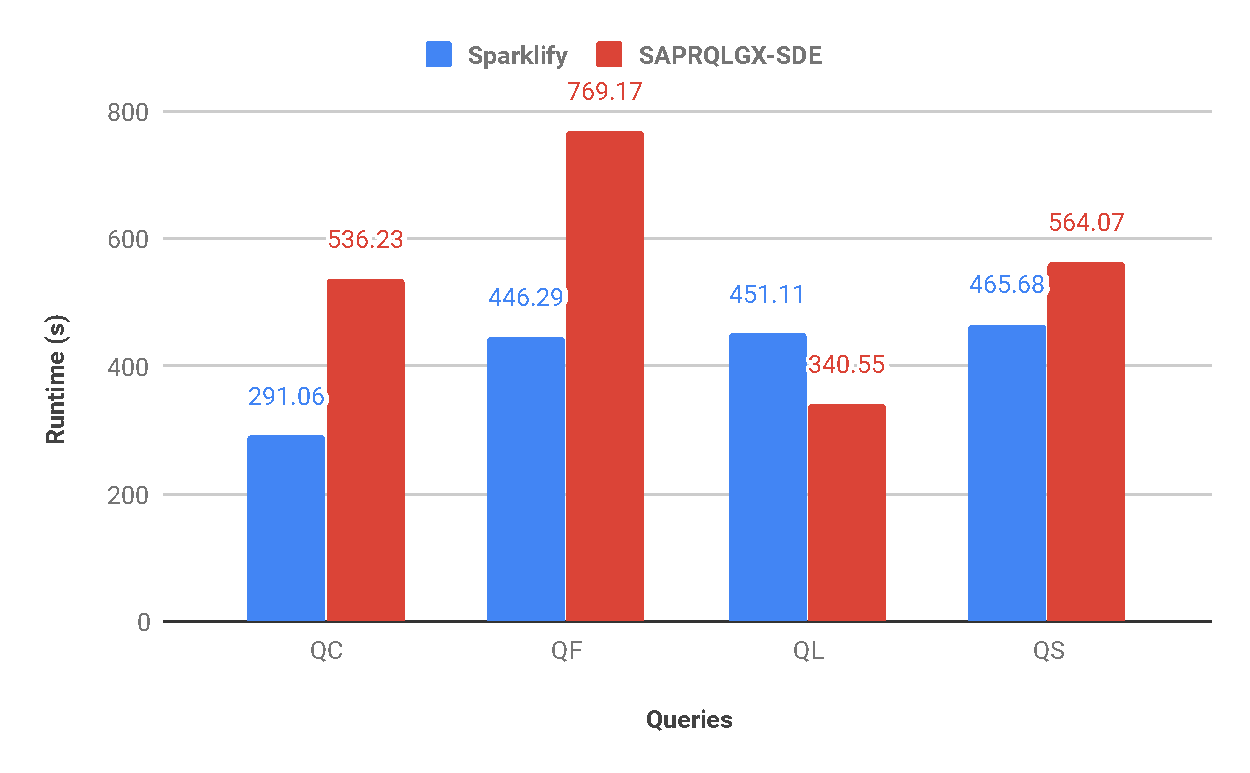
\includegraphics[width=1.0\columnwidth]{images/6_scalable_rdf_querying/sparklify-overall-analysis.pdf}
    \caption{\textbf{Overall analysis of queries on Watdiv-100M dataset (cluser mode)}.
    This analysis gives more insights about running Watdiv queries on \textit{Watdiv-100M} dataset in a cluster mode on both approaches, Sparklify and SPARQLGX-SDE.
    The findings show that SPARQLGX-SDE performance decreases as the number of triple patterns involved in the query increase.
    In contrast to SPARQLGX-SDE, Sparklify seems to perform well when there are more triple pattern involved (i.e. \textit{QC}, \textit{QF} and \textit{QS}) but slightly worst when there are linear queries (see \textit{QL}) evaluated. }
    \label{fig:sparklify-overall-analysis}
\end{figure}

According to Figure~\ref{fig:sparklify-overall-analysis}, SPARQLGX-SDE performance decreases as the number of triple patterns involved in the query increase.
This might be due to the fact that SPARQLGX-SDE has to read the whole triple file each time.
In contrast to SPARQLGX-SDE, Sparklify seems to perform well when there are more triple pattern involved (see queries \textit{QC}, \textit{QF} and \textit{QS} in the Figure~\ref{fig:sparklify-overall-analysis}) but slightly worst when there are linear queries (see \textit{QL}) evaluated. 
This may be due to the reason that Sparqlify typically rewrites a \gls{SPARQL} query into a single SQL query, thus maximizing the opportunities given to the Spark SQL optimizer. Conversely, SPARQLGX-SDE constructs the workflow by chaining Scala API calls, which may restrict the possibilities e.g. in regard to join ordering.
Based on our findings and the evaluation study carried out in this paper, we show that Sparklify is scalable and the execution time ends in a reasonable time given the size of the dataset.

%----Semantic-based approach--------

\section{A Scalable Semantic-based Distributed Approach for SPARQL query evaluation}
\label{sec:semantic-based-approach}

In this section, we present the system architecture of the Semantic-based approach, the semantic-based partitioning, and mapping \gls{SPARQL} to Spark Scala-compliant code.

\subsection{System Architecture Overview}
The system architecture overview is shown in the Figure~\ref{fig:semantic-based-architecture}.

\begin{figure*}
\centering
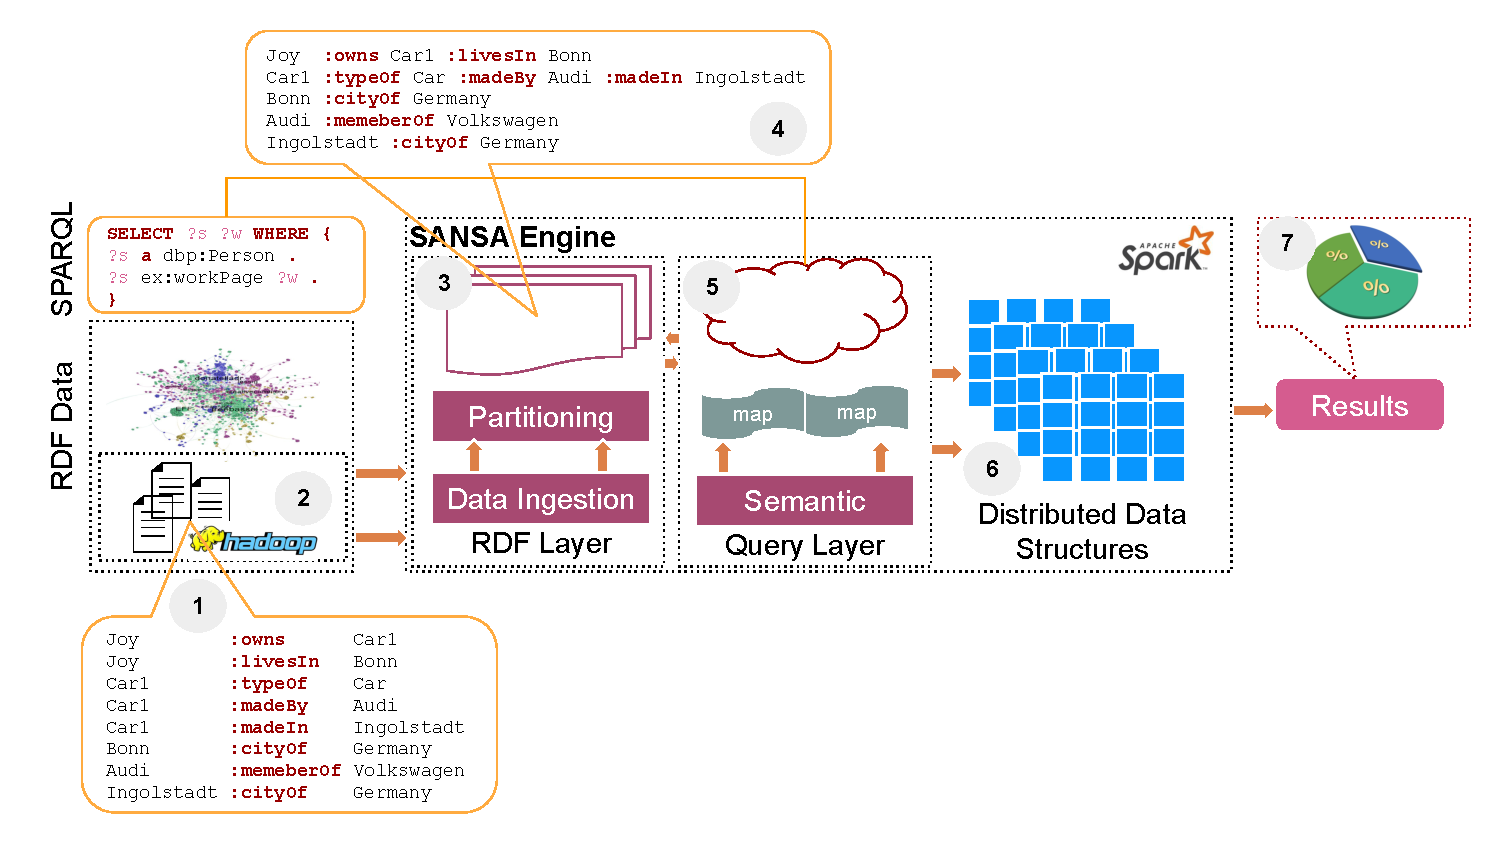
\includegraphics[width=1.0\columnwidth]{images/6_scalable_rdf_querying/semantic-based-architecture.pdf}
\caption{\textbf{Semantic-based System Architecture Overview}.
It consists of three main facets: Data Storage Model -- model and partition the data using the semantic-based approach, SPARQL Query Fragments Translator -- the process of generating the Scala code in the format of Spark RDD operations, and Query Evaluator -- the SPARQL evaluation using the Spark RDD executable code (generated from the previous step).}
\label{fig:semantic-based-architecture}
% source : https://docs.google.com/presentation/d/14KAs3q_gfB9iTR6ZrIrzrLGU19-A_UUbqO1Xaz84auw
\end{figure*}

It consists of three main facets: Data Storage Model, \gls{SPARQL} Query Fragments Translator, and Query Evaluator.
Below, each facet is discussed in more details.

\subsubsection{Data Storage Model}
We model the \gls{RDF} data following the concept of \gls{RDD}s. 
\gls{RDD}s are immutable collections of records, which represent the basic building blocks of the Spark framework.
\gls{RDD}s can be kept in-memory and are able to operate in parallel throughout the Spark cluster.
We make use of SANSA~\cite{lehmann-2017-sansa-iswc}'s data representation and distribution layer for such representation.

\defn{Data Partitioning}
Partitioning the \gls{RDF} data is the process of dividing datasets in a specific logical and/or physical representation in order to ease faster access and better maintenance.
Often, this process is performed for improving the system availability, load balancing and query processing time.
There are many different data partitioning techniques proposed in the literature. 
We choose to investigate the so-called \textit{semantic-based partitioning} behaviors when dealing with large-scale \gls{RDF} datasets.
This partitioned technique was proposed in the SHARD~\cite{Rohloff2010SHARD} system.
We have implemented this technique using in-memory processing engine, Apache Spark for better performance.
A semantically partitioned fact is a tuple $(S, R)$ containing pieces of information $R \in (P, O)$ about the same $S$ where $S$ is a unique subject on the \gls{RDF} graph and $R$ represents all its associated facts i.e predicates $P$ and objects $O$.

\defn{Data Model}
First, the \gls{RDF} data (see \textit{Step 1} as an example) needs to be loaded into a large-scale distributed storage (\textit{Step 2}).
We use \gls{HDFS}.
We choose \gls{HDFS} as Spark is capable of performing operations based on data locality in order to choose the nearest data for faster and efficient computation over the cluster.
Second, we partition (\textit{Step 3}) the data using semantic-based partitioning (see \textit{Step 4} as an example of such partition).
Instead of working with table-wise representation where the triples are kept in the format of $\verb|RDD<Triple>|$, data is partitioned into subject-based grouping (e.g. all entities which are associated with a unique subject).
Consider the example in the Figure~\ref{fig:semantic-based-architecture} (\textit{Step 2}, first line), which represents two triples associated with the entity \verb|Joy|:
$$\verb|Joy :owns Car1 :livesIn Bonn|$$
This line represents that the entity \verb|Joy| owns a car entity \verb|Car1|, and that \verb|Joy| lives in \verb|Bonn|.

Often flattening data is considered immature with respect to other data representation, we want to explore and investigate if it improves the performance of the query evaluation.
We choose this representation for the reason of easy-storage and reuse while designing a query engine. 
Although, it slightly degrades the performance when it comes to multiple scans over the table when there are multiple predicates involved in the query. However, this is minimal, as Spark uses in-memory, caching operations.
We will discuss this on the Section~\ref{sec:semantic-based-evaluation} into more detail.

\subsubsection{SPARQL Query Fragments Translation}
This process generates the Scala code in the format of Spark \gls{RDD} operations using the key-value pairs mechanism.
With Spark pairRDD, one can manipulate the data by splitting it into key-value pairs and group all associated values with the same keys. 
It walks through the \gls{SPARQL} query (\textit{Step 4}) using the Jena ARQ\furl{https://jena.apache.org/documentation/query/} and iterate through clauses in the \gls{SPARQL} query and bind the variables into the \gls{RDF} data while fulfilling the clause conditions.
Such iteration corresponds to a single clause with one of the Spark operations (e.g. \emph{map}, \emph{filter}, \emph{reduce}).
Often this operation needs to be materialized i.e the result set of the next iteration depends on the previous clauses and therefore a \emph{join} operation is needed.
This is a bottleneck since scanning and shuffling is required.
In order to keep these joins as small as possible, we leverage the caching techniques of the Spark framework by keeping the intermediate results in-memory while the next iteration is performed.
Finally, the Spark-Scala executable code is generated (\textit{Step 5}) using the bindings corresponding the query.
Besides simple \gls{BGP} translation, our system supports \emphb{UNION}, \emphb{LIMIT} and \emphb{FILTER} clauses.

\subsubsection{Query Evaluator}
The mappings created as shown in the previous section can now be evaluated directly into the Spark \gls{RDD} executable code.
The result set of these operations is distributed data structure of Spark (e.g. \gls{RDD}) (\textit{Step 6}).
The result set can be used for further processing and visualization using the SANSA-Notebooks (\textit{Step 7})~\cite{iermilov-2017-sansa-iswc-demo}.


\subsection{Distributed Algorithm Description}
\label{subsection:semantic-based-algorithm}
We implement our approach using the Apache Spark framework (see Algorithm~\ref{alg:semantic-based-algorithm}). 
It constructs the graph (\textit{Line \ref{line:semantic-based-rdf2rdd}}) while reading \gls{RDF} data and converts it into an \gls{RDD} of triples.
Later, it partitions the data (\textit{Line \ref{line:semantic-based-partitionGraph}}, for more details see Algorithm~\ref{alg:semantic-based-partitionGraph}) using the semantic-based partitioning (SP) strategy.
Finally, the query evaluator is constructed (\textit{Line \ref{line:semantic-based-sparql}}) which is detailed in Algorithm~\ref{alg:semantic-based-sparql}.

\begin{algorithm*}
\caption{Spark parallel semantic-based query engine.}
\label{alg:semantic-based-algorithm}
\SetKwInOut{Input}{input}\SetKwInOut{Output}{output}
\Input{$q$: a SPARQL query, $input$: an RDF dataset}
\Output{$result$ an RDD -- list of result set}
    \tcc{Loading the graph}
    $\textit{graph} = spark.\textbf{rdf}(lang)(input)$ \label{line:semantic-based-rdf2rdd}\\
    \tcc{Partitioning the graph. See Algorithm~\ref{alg:semantic-based-partitionGraph} for more details.}
    $partitionGraph \leftarrow graph.\textbf{partitonAsSemanticGraph}()$ \label{line:semantic-based-partitionGraph}\\
     \tcc{Querying the graph. See Algorithm~\ref{alg:semantic-based-sparql} for more details.}
    $result \leftarrow partitionGraph.\textbf{sparql}(q)$ \label{line:semantic-based-sparql}\\
\Return{$result$}
\end{algorithm*}

The partition algorithm (see Algorithm~\ref{alg:semantic-based-partitionGraph}) transforms the \gls{RDF} graph into a convenient SP (\textit{Line \ref{line:semantic-based-partitionGraph}}).
For each unique triple in the graph in a distributed fashion, it does the following: It gets the values about subjects and objects (\textit{Line \ref{line:semantic-based-subject_object_values}}) and local name of the predicate (\textit{Line \ref{line:semantic-based-predicate}}).
It generates the key-value pairs of the subject and its associated triples with predicate and object separated with the space in between (\textit{Line \ref{line:semantic-based-partition_data}}).
After the mapping is done, the data is grouped by key (in our case \emph{subject}) (\textit{Line \ref{line:semantic-based-groupBy}}).
Afterward, when this information is collected, the block is partitioned using the \emph{map} transformation function of Spark to refactor the format of the lines based on the above information (\textit{Line \ref{line:semantic-based-partitionGraph_map}}).

\begin{algorithm*}
\caption{\textbf{partitonAsSemanticGraph}: Semantic-based partition algorithm.}
\label{alg:semantic-based-partitionGraph}
\SetKwInOut{Input}{input}\SetKwInOut{Output}{output}
\Input{$graph$: an RDD of triples}
\Output{$partionedData$: an RDD of partitions}
$partitonedData \leftarrow \emptyset $\\
    \ForEach{ $ \forall! triple \in graph\quad \&\& \quad triple.getSubject \neq \emptyset $}{
        $s \leftarrow triple.getSubject; \quad o \leftarrow triple.getObject$ \label{line:semantic-based-subject_object_values}\\
        $p \leftarrow triple.getPredicate.getLocalName$ \label{line:semantic-based-predicate}\\
            $partitonedData~+=(s,~p + "~" + o + "~" )$ \label{line:semantic-based-partition_data}
            }
        $partitonedData.reduceByKey(\_+\_)$\label{line:semantic-based-groupBy}\\
        \quad \quad \quad \quad \quad \quad $.map(f\rightarrow(f.\_1 + "~" + f.\_2))$ \label{line:semantic-based-partitionGraph_map}\\
\Return{$partitonedData$}
\end{algorithm*}


This \gls{SPARQL} query rewriter includes multiple Spark operations.
First, partitioned data is mapped to a list of variable bindings satisfying the first \gls{BGP} of the query (\textit{Line \ref{line:semantic-based-firstVariable}}). 
During this process, the duplicates are removed and the intermediate result is kept in-memory (\gls{RDD}) with the variable bindings as a key.
The consequent step is to iterate through other variables and bind them by processing the upcoming query clauses and/or filtering the other ones unseen on the new clause.
These intermediate steps perform Spark operations over both, the partitioned data and the previously bound variables which were kept on Spark \gls{RDD}s.

The \textit{i}th step discovers all variables in the partitioned data which satisfy the \textit{i}th clause appeared and keep this intermediate result in-memory with the key being any variable in the \textit{i}th step which has been introduced on the previous step.
During this iteration, the intermediate results are reconstructed in the way that the variables not seen in this iteration are mapped (\textit{Line \ref{line:semantic-based-mapByKey}}) with the variables of the previous clause and generate a key-value pair of variable bindings.
Afterward, the \emph{join} operation is performed over the intermediate results from the previous clause and the new ones with the same key.
This process iterates until all clauses are seen and variables are assigned.
Finally, the variable binding (\textit{Line \ref{line:semantic-based-filter_variables}}) to fulfill the \emph{SELECT} clause of the \gls{SPARQL} query happens and returns the result (\textit{Line \ref{line:semantic-based-result}}) of only those variables which are present in the SELECT clause.

\begin{algorithm*}
\caption{\textbf{sparql}: Semantic-based query algorithm.}
\label{alg:semantic-based-sparql}
\SetKwInOut{Input}{input}\SetKwInOut{Output}{output}
\Input{partitonedData: an RDD of partitions}
\Output{$result$ an RDD of result set}
    \ForEach{$p \in partitionedData$}{
        $1stVariable \leftarrow assignVariablesFor1stClaues()$\label{line:semantic-based-firstVariable}\\
        \ForEach{$i \in getClauses()$}{
        $iVariable \leftarrow assignVariablesForiClaues()$\\
        $mapResult \leftarrow mapByKey(getCommonVariables())$\label{line:semantic-based-mapByKey}\\
        $joinResult \leftarrow join(mapResult)$
        }
    $joinResult.filter(getSelectVariables())$ \label{line:semantic-based-filter_variables}\\
    $result \leftarrow result.join(joinResult)$ \label{line:semantic-based-result}\\
  }
\Return{$result$}
\end{algorithm*}

\subsection{Evaluation}
\label{sec:semantic-based-evaluation}

In our evaluation, we observe the impact of semantic-based partitioning and analyze the scalability of our approach when the size of the dataset increases.

In the following subsections, we present the benchmarks used along with the server configuration setting, and finally, we discuss our findings.

\subsubsection{Experimental Setup}
We make use of two well-known \gls{SPARQL} benchmarks for our experiments: 
the \textit{Waterloo \gls{SPARQL} Diversity Test Suite (WatDiv)} v0.6~\cite{Alu2014DiversifiedST} and \textit{Lehigh University Benchmark (LUBM)} v3.1~\cite{Guo2005LUBMAB}.
The dataset characteristics of the considered benchmarks are given in Table~\ref{tab:semantic-based-dataset_info}.

\textit{WatDiv} comes with a test suite with different query shapes which allows us to compare the performance of our approach and the other approaches. 
In particular, it comes with a predefined set of 20 query templates which are grouped into four categories, based on the query shape: \textit{star-shaped} queries, \textit{linear-shaped} queries, \textit{snowflake-shaped} queries, and \textit{complex-shaped} queries.
We have used \textit{WatDiv} datasets with 10M to 100M triples with scale factors 10 and 100, respectively.
In addition, we have generated the \gls{SPARQL} queries using \textit{WatDiv Query Generator}.

\textit{LUBM} comes with a \textit{Data Generator (UBA)} which generates synthetic data over the \textit{Univ-Bench} ontology in the unit of a university. 
\textit{LUBM} provides Test Queries, more specifically 14 test queries.
Our \textit{LUBM} datasets consist of 1000, 2000, and 3000 universities.
The number of triples varies from 138M for 1000 universities, to 414M triples for 3000 universities.


\begin{table*}
\centering
\begin{tabularx}{\textwidth}{Xcccccc}	
\toprule
\multirow{2}{*}{} & \multicolumn{3}{c|}{LUBM} & \multicolumn{3}{c}{Watdiv} \\
\cline{2-7}  \rule{0pt}{10pt}
&   \scriptsize{1K} & \scriptsize{2K} & \scriptsize{3K} & \scriptsize{10M} &\scriptsize{100M} &\\
\midrule
\scriptsize{\#nr. of triples}& \scriptsize{138,280,374} & \scriptsize{276,349,040} & \scriptsize{414,493,296}  &  \scriptsize{10,916,457} & \scriptsize{108,997,714} &  \\
\scriptsize{size (GB)}  & \scriptsize{24} & \scriptsize{49}  & \scriptsize{70} & \scriptsize{1.5} &\scriptsize{15} &\\
\bottomrule
\end{tabularx}
{\caption{\textbf{Dataset characteristics (nt format)}.
Lists dataset information used on the evaluation.
The size (in GB) and the number of triples are given.}
\label{tab:semantic-based-dataset_info}}
\end{table*}

We implemented our approach using Spark-2.4.0, Scala 2.11.11, Java 8, and all the data were stored on the \gls{HDFS} cluster using Hadoop 2.8.0.
All experiments were carried out on a commodity cluster of 6 nodes (1 master, 5 workers): Intel(R) Xeon(R) CPU E5-2620 v4 @ 2.10GHz (32 Cores), 128 GB RAM, 12 TB SATA RAID-5.
We executed each experiment three times and the average query execution time has been reported.

\subsubsection{Preliminary Results}
We run experiments on the same cluster and evaluate our approach using the above benchmarks. 
In addition, we compare our proposed approach with selected state-of-the-art distributed \gls{SPARQL} query evaluators.
In particular, we compare our approach with SHARD~\cite{Rohloff2010SHARD} -- the original approach implemented on Hadoop MapReduce, \emph{SPARQLGX}~\cite{sparqlgx-iswc-2016}'s direct evaluator SDE, and Sparklify~\cite{2019-sansa-sparklify-iswc} and report the query execution time (cf.\ Table~\ref{tbl:semantic-based-performance-analysis}).
We have selected these approaches as they do not include any pre-processing steps (e.g. statistics) while evaluating the \gls{SPARQL} query, similar to our approach.

Our evaluation results for performance analysis, sizeup analysis, node scalability, and breakdown analysis by \gls{SPARQL} queries are shown in Table~\ref{tbl:semantic-based-performance-analysis}, Figure~\ref{fig:semantic-based-sizeup-scalability}, \ref{fig:semantic-based-node-scalability}, and \ref{fig:semantic-based-overall-analysis} respectively.
In Table\ref{tbl:semantic-based-performance-analysis} we use ``fail'' whenever the system fails to complete the task and ``n/a'' when the task could not be completed due to a parser error (e.g.\ not able to translate some of the basic patterns to \gls{RDD}s operations).

In order to evaluate our approach with respect to the \textit{speedup}, we analyze and compare it with other approaches.

This set of experiments was run on three datasets, \emph{Watdiv-10M}, \emph{Watdiv-100M} and \emph{LUBM-1K}.

\begin{table*}[t]
\centering
\begin{tabularx}{\textwidth}{*{5}{X}}	
\toprule
\multicolumn{1}{l}{}& \multicolumn{4}{c}{\scriptsize{Runtime (s)} (\scriptsize{mean})} \\
\cline{2-5}
\rule{0pt}{4pt}
\multirow{1}{*}{\scriptsize{\textbf{Queries}}} & \multicolumn{1}{c|}{\scriptsize{\textbf{SHARD}}} & \multicolumn{1}{c|}{\scriptsize{\textbf{SPARQLGX-SDE}}} & \multicolumn{1}{c|}{\scriptsize{\textbf{SANSA.Sparklify}}} & \multicolumn{1}{c}{\scriptsize{\textbf{SANSA.Semantic}}} \\
\midrule
\multirow{5}{*}{\rotatebox{90}{\scriptsize{\textbf{Watdiv-10M}}}}
&  & & & \\
\hspace{0.2cm} $C3$ & \textcolor{blue}{\scriptsize{n/a}} & \win \scriptsize{38.79} & \scriptsize{72.94} &  \scriptsize{90.48} \\
\hspace{0.2cm} $F3$ & \textcolor{blue}{\scriptsize{n/a}}& \win \scriptsize{38.41} & \scriptsize{74.69} & \textcolor{blue}{\scriptsize{n/a}} \\
\hspace{0.2cm} $L3$ & \textcolor{blue}{\scriptsize{n/a}}  & \scriptsize{21.05} & \scriptsize{73.16} & \scriptsize{72.84} \\
\hspace{0.2cm} $S3$ & \textcolor{blue}{\scriptsize{n/a}}  & \win \scriptsize{26.27} & \scriptsize{70.1} & \scriptsize{79.7} \\
\midrule
\multirow{5}{*}{\rotatebox{90}{\scriptsize{\textbf{Watdiv-100M}}}}
&  & & & \\
\hspace{0.2cm}  $C3$ & \textcolor{blue}{\scriptsize{n/a}} & \scriptsize{181.51} & \win \scriptsize{96.59} & \scriptsize{300.82} \\
\hspace{0.2cm} $F3$ & \textcolor{blue}{\scriptsize{n/a}} & \scriptsize{162.86} & \scriptsize{91.2} &  \textcolor{blue}{\scriptsize{n/a}}\\
\hspace{0.2cm} $L3$ & \textcolor{blue}{\scriptsize{n/a}} & \scriptsize{84.09} & \win \scriptsize{82.17} & \scriptsize{189.89} \\
\hspace{0.2cm} $S3$ & \textcolor{blue}{\scriptsize{n/a}}  & \scriptsize{123.6} & \win \scriptsize{93.02}  & \scriptsize{176.2}\\
\midrule
\multirow{14}{*}{\rotatebox{90}{\scriptsize{\textbf{LUBM-1K}}}}
$Q1$ & \scriptsize{774.93} & \scriptsize{103.74} & \win \scriptsize{103.57} & \scriptsize{226.21}\\
\hspace{0.2cm} $Q2$ & \textcolor{red}{\scriptsize{fail}} & \textcolor{red}{\scriptsize{fail}} &  \scriptsize{3348.51} & \win \scriptsize{329.69}\\
\hspace{0.2cm} $Q3$ & \scriptsize{772.55} & \scriptsize{126.31} & \win \scriptsize{107.25} & \scriptsize{235.31} \\
\hspace{0.2cm} $Q4$ & \scriptsize{988.28} & \scriptsize{182.52} & \win \scriptsize{111.89} & \scriptsize{294.8} \\
\hspace{0.2cm} $Q5$ & \scriptsize{771.69} & \scriptsize{101.05} & \win \scriptsize{100.37} & \scriptsize{226.21} \\
\hspace{0.2cm} $Q6$ & \textcolor{red}{\scriptsize{fail}} & \win \scriptsize{73.05} & \scriptsize{100.72} & \scriptsize{207.06} \\
\hspace{0.2cm} $Q7$ & \textcolor{red}{\scriptsize{fail}} & \scriptsize{160.94} & \win \scriptsize{113.03} & \scriptsize{277.08} \\
\hspace{0.2cm} $Q8$ & \textcolor{red}{\scriptsize{fail}} & \scriptsize{179.56} & \win \scriptsize{114.83} & \scriptsize{309.39} \\
\hspace{0.2cm} $Q9$ & \textcolor{red}{\scriptsize{fail}} & \scriptsize{204.62} & \win \scriptsize{114.25} & \scriptsize{326.29} \\
\hspace{0.2cm} $Q10$ & \scriptsize{780.05} & \win \scriptsize{106.26} & \scriptsize{110.18} & \scriptsize{232.72} \\
\hspace{0.2cm} $Q11$ & \scriptsize{783.2} & \scriptsize{112.23} & \win \scriptsize{105.13} & \scriptsize{231.36}\\
\hspace{0.2cm} $Q12$ & \textcolor{red}{\scriptsize{fail}} & \scriptsize{159.65} & \win \scriptsize{105.86} & \scriptsize{283.53}\\
\hspace{0.2cm} $Q13$ & \scriptsize{778.16} & \scriptsize{100.06} & \win \scriptsize{90.87} & \scriptsize{220.28} \\
\hspace{0.2cm} $Q14$ & \scriptsize{688.44} & \win \scriptsize{74.64} & \scriptsize{100.58} & \scriptsize{204.43}\\
\bottomrule
\end{tabularx}
{\caption{\textbf{Performance analysis on large-scale RDF datasets}.
An comparison of our approach with SHARD – the original approach implemented on Hadoop MapReduce, SPARQLGX’s direct evaluator SDE, and Sparklify w.r.t query execution time.
}
\label{tbl:semantic-based-performance-analysis}}
\end{table*} %source : https://docs.google.com/spreadsheets/d/1pGLuknI6EsTApGEZHqPhN4VEFBa63vVpNpA4r4BYXbQ

Table~\ref{tbl:semantic-based-performance-analysis} presents the performance analysis of the systems on three different datasets.
We can see that our approach evaluates most of the queries as opposed to SHARD.
SHARD system fails to evaluate most of the \textit{LUBM} queries and its parser does not support \textit{Watdiv} queries.
On the other hand, SPARQLGX-SDE performs better than both Sparklify and our approach, when the size of the dataset is considerably small (e.g. less than 25GB).
This behavior is due to the large partitioning overhead for Sparklify and our approach.
However, Sparklify performs better compared to SPARQLGX-SDE when the size of the dataset increases (see \textit{Watdiv-100M} results in the Table~\ref{tbl:semantic-based-performance-analysis}) and the queries involve more joins (see \textit{LUBM-1K} results in the Table~\ref{tbl:semantic-based-performance-analysis}).
This is due to the Spark SQL optimizer and Sparqlify self-joins optimizers.
Both SHARD and SPARQLGX-SDE fail to evaluate query \textit{Q2} in the \textit{LUBM-1K} dataset. 
Sparklify can evaluate the query but takes longer as compared to our approach.
This is due to the fact that our approach uses Spark's lazy evaluation and join optimization by keeping the intermediate results in memory.

~\\\defn{Scalability analysis}
In order to evaluate the scalability of our approach, we conducted two sets of experiments.
First, we measure the data scalability (e.g.\ size-up) of our approach and position it with other approaches.
As SHARD fails for most of the LUBM queries, we omit other queries on this set of experiments and choose only Q1, Q5, and Q14.
Q1 has been chosen due to its complexity while bringing large inputs of the data and high selectivity, Q5 since it has considerably larger intermediate results due to the triangular pattern in the query, and Q14 mainly for its simplicity.
We run experiments on three different sizes of \textit{LUBM} (see Figure~\ref{fig:semantic-based-sizeup-scalability}).

\begin{figure*}
 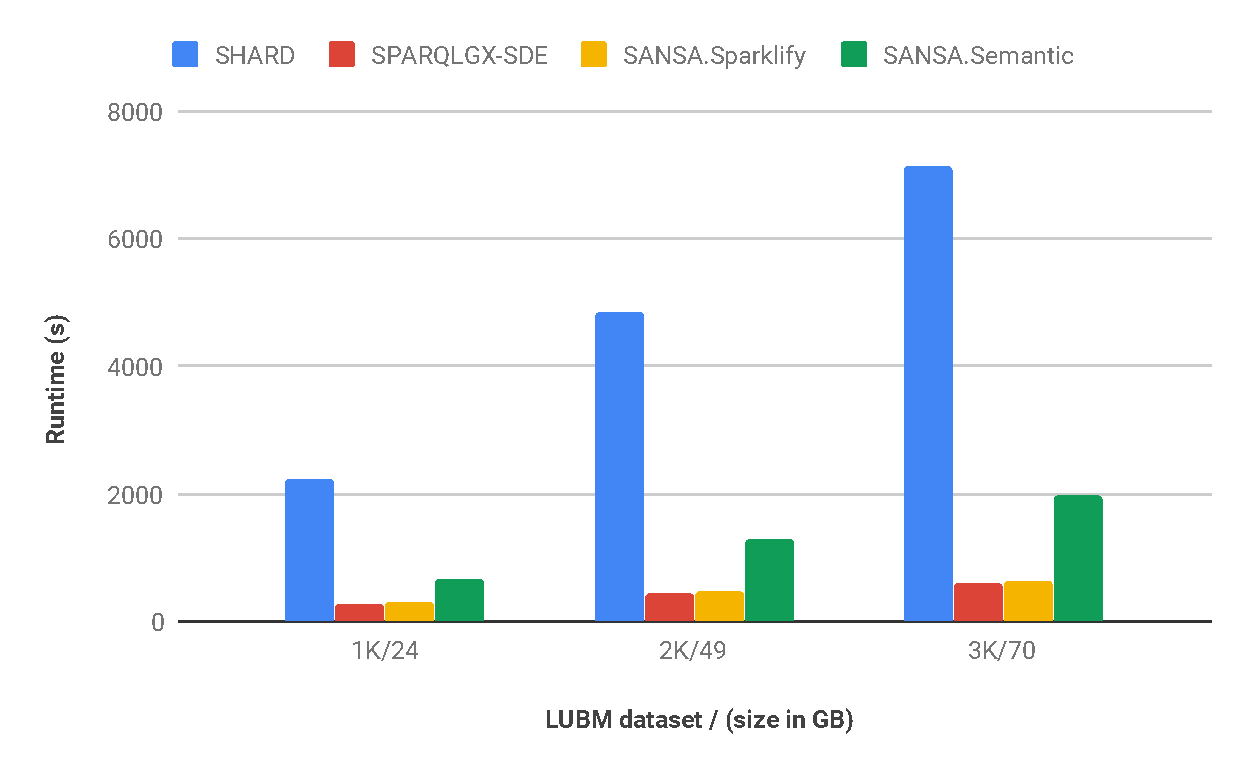
\includegraphics[width=1.0\columnwidth]{images/6_scalable_rdf_querying/semantic-based-sizeup-scalability.pdf}
    \caption{\textbf{Sizeup analysis (on LUBM dataset)}.
    The analysis keep the number of nodes constant i.e. 5 worker nodes and increase the size of the datasets to measure whether semantic-based approach deals with larger datasets.
    The query execution time for our approach grows linearly when the size of the datasets increases.
    This shows the scalability of our approach as compared to SHARD, in context of the sizeup.
    SHARD suffers from the expensive overhead of MapReduce joins which impact its performance, as a result, it is significantly worse than other systems.
    }
    \label{fig:semantic-based-sizeup-scalability}
\end{figure*}

We keep the number of nodes constant i.e.\ 5 worker nodes and increase the size of the datasets to measure whether our approach deals with larger datasets.

We see that the query execution time for our approach grows linearly when the size of the datasets increases.
This shows the scalability of our approach as compared to SHARD, in context of the sizeup.
SHARD suffers from the expensive overhead of MapReduce joins which impact its performance, as a result, it is significantly worse than other systems.

Second, in order to measure the node scalability of our approach, we increase the number of worker nodes and keep the size of the dataset constant.
We vary them from 1, 3 to 5 worker nodes.

\begin{figure*}
  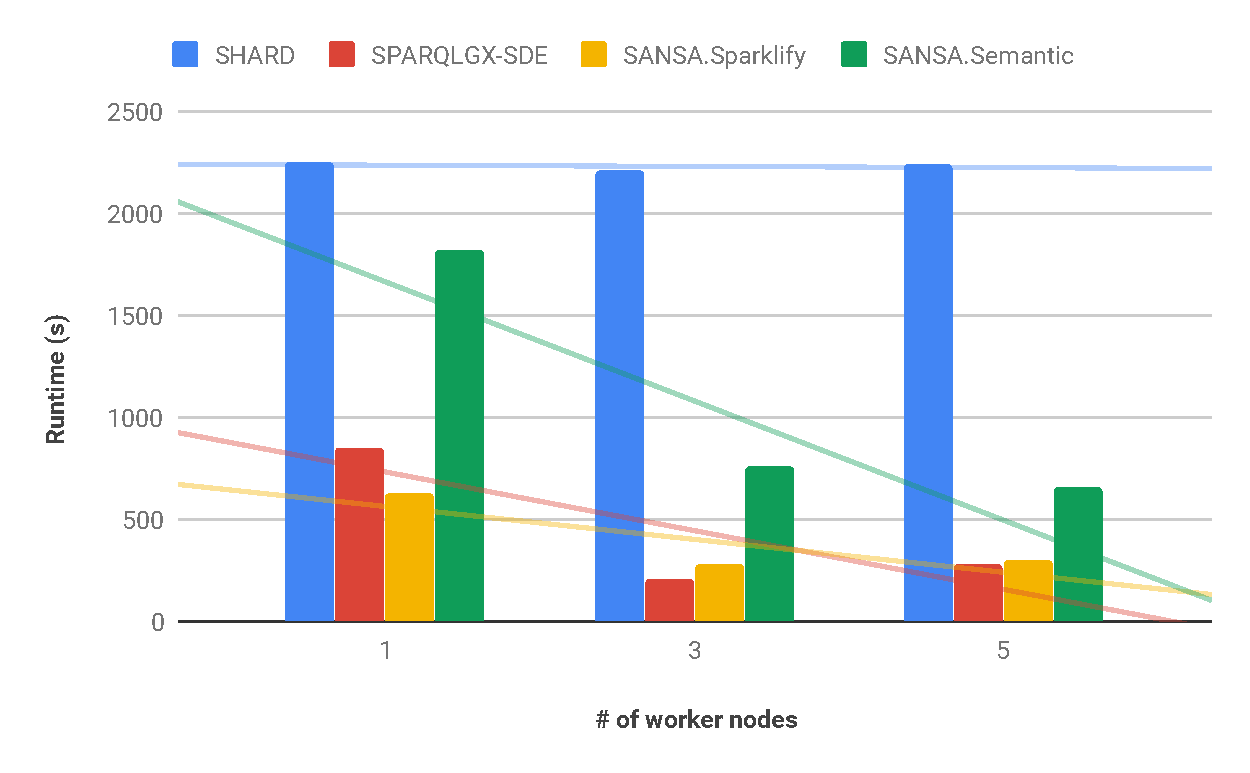
\includegraphics[width=1.0\columnwidth]{images/6_scalable_rdf_querying/semantic-based-node-scalability.pdf}
    \caption{\textbf{Node scalability (on LUBM-1K)}.
     The analysis increase the number of worker nodes and keep the size of the dataset constant. 
    We vary them from 1, 3 to 5 worker nodes.
    As the number of nodes increases, the runtime cost of our query engine decreases linearly as compared with the SHARD, which keeps staying constant. 
    SHARD performance stays constant (high) even when more worker nodes are added. This trend is due to the communication overhead SHARD needs to perform between map and reduce steps. The execution time of our approach decreases about 1.7 times (from 1,821.75 seconds down to 656.85 seconds) as the worker nodes increase from one to five nodes.}
    \label{fig:semantic-based-node-scalability}
\end{figure*}

Figure~\ref{fig:semantic-based-node-scalability} shows the performance of systems on \textit{LUBM-1K} dataset when the number of worker nodes varies.
We see that as the number of nodes increases, the runtime cost of our query engine decreases linearly as compared with the SHARD, which keeps staying constant.
SHARD performance stays constant (high) even when more worker nodes are added.
This trend is due to the communication overhead SHARD needs to perform between map and reduce steps.
The execution time of our approach decreases about 1.7 times (from 1,821.75 seconds down to 656.85 seconds) as the worker nodes increase from one to five nodes.
SPARQLGX-SDE and Sparklify perform better when the number of nodes increases compared to our approach and SHARD. 

Our main observation here is that our approach can achieve linear scalability in the performance.

~\\ \defn{Correctness}
In order to assess the correctness of the result set, we computed the count of the result set for the given queries and compare it with other approaches.
As a result of it, we conclude that all approaches return exactly the same result set.
This implies the correctness of the results.

~\\ \defn{Breakdown by \gls{SPARQL} queries}
Here we analyze some of the LUBM queries (Q1, Q5, Q14) run on a \textit{LUBM-1K} dataset in a cluster mode on all the systems.

\begin{figure*}
   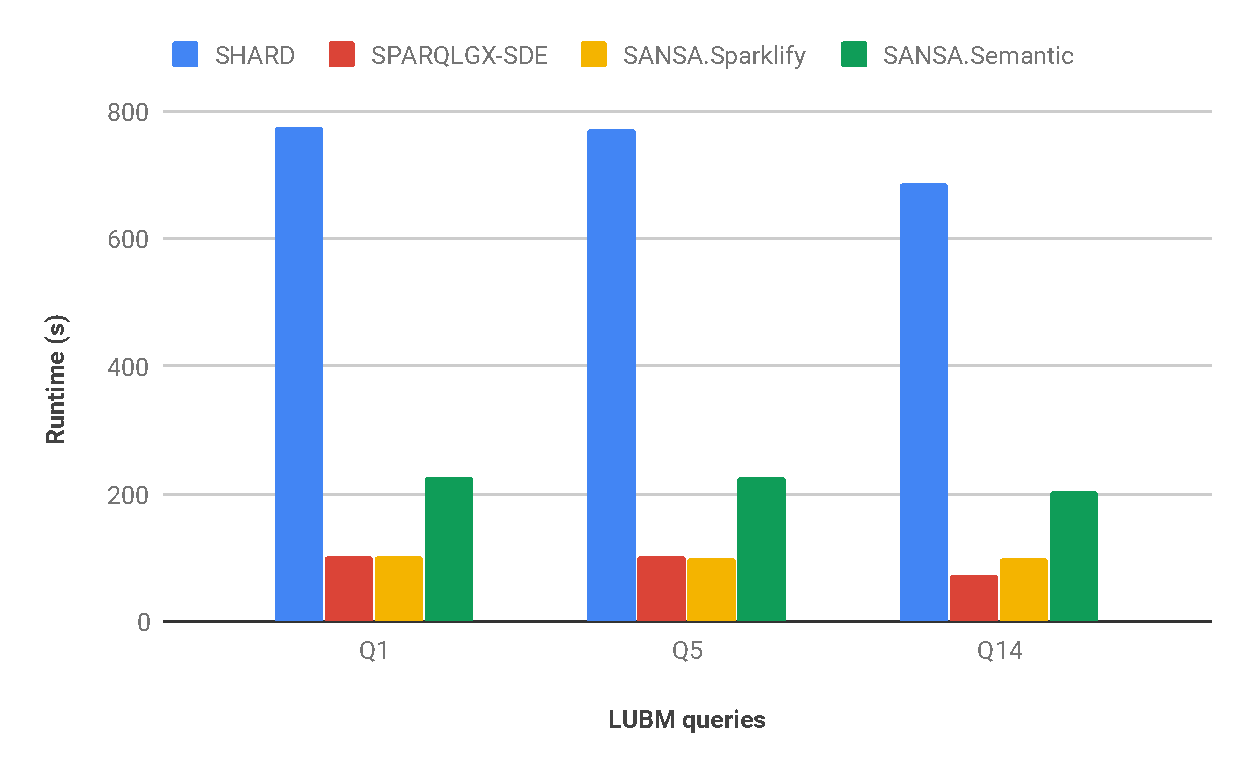
\includegraphics[width=1.0\columnwidth]{images/6_scalable_rdf_querying/semantic-based-overall-analysis.pdf}
    \caption{\textbf{Overall analysis of queries on LUBM-1K dataset (cluser mode)}.
    This analysis depict some of LUBM queries (Q1, Q5, Q14) run on a \textit{LUBM-1K} dataset in a cluster mode on all the systems. 
    Overall, our approach performs better compared to Hadoop-based system, SHARD due to the use of the Spark framework which leverages the in-memory computation for faster performance.
    However, the performance declines as compared to other approaches which use vertical partitioning (e.g., SPARQLGX-SDE on RDD and Sparklify on Spark SQL).
    This is due to the fact that our approach performs de-duplication of triples that involves shuffling and incurs network overhead.
    }
    \label{fig:semantic-based-overall-analysis}
\end{figure*}

We can see from Figure~\ref{fig:semantic-based-overall-analysis} that our approach performs better compared to Hadoop-based system, SHARD. 
This is due to the use of the Spark framework which leverages the in-memory computation for faster performance.
However, the performance declines as compared to other approaches which use vertical partitioning (e.g., SPARQLGX-SDE on \gls{RDD} and Sparklify on Spark SQL).
This is due to the fact that our approach performs de-duplication of triples that involves shuffling and incurs network overhead.
The results show that the performance of SPARQLGX-SDE decreases as the number of triple patterns involved in the query increases (see \textit{Q5}) when compared to Sparklify. 
However, SPARQLGX-SDE performs better when there are simple queries (see \textit{Q14}). 
This occurs because SPARQLGX-SDE must read the whole RDF graph each time when there is a triple pattern involved.
In contrast to SPARQLGX-SDE, Sparklify performs better when there are more triple patterns involved (see \textit{Q5}) but slightly worse when linear queries (see \textit{Q14}) are evaluated. 

Based on our findings and the evaluation study carried out, we show that our approach can scale up with the increasing size of the dataset.

\section{Summary}
\label{sec:scalable-rdf-querying-summary}
Querying \gls{RDF} data becomes challenging when the size of the data increases.
Existing Spark-based \gls{SPARQL} systems mostly
do not retain all \gls{RDF} term information consistently while transforming them to a dedicated storage model such as using vertical partitioning.
Often, this process is both data and computing intensive and raises the need for a scalable, efficient and comprehensive query engine which can handle large scale \gls{RDF} datasets.

In this chapter, we propose scalable approaches for \gls{SPARQL} query evaluation over distributed \gls{RDF} data. 
First, \emph{Sparklify}: a scalable software component for efficient evaluation of \gls{SPARQL} queries over distributed \gls{RDF} datasets. 
It uses Sparqify as a SPARQL-to-SQL rewriter for translating \gls{SPARQL} queries into Spark executable code.
By doing so, it leverages the advantages of the Spark framework.
SANSA features methods to execute \gls{SPARQL} queries directly as part of Spark workflows instead of writing the code corresponding to those queries (sorting, filtering, etc.).
It also provides a command-line interface and a \gls{W3C} standard compliant \gls{SPARQL} endpoint for externally querying data that has been loaded using the SANSA framework.
We have shown empirically that Sparklify can scale horizontally and perform well w.r.t to the state-of-the-art approaches.

With this work, we showed that the application of OBDA tooling to Big Data frameworks achieves promising results in terms of scalability. 
We present a working prototype implementation that can serve as a baseline for further research.

As a second approach, we investigated and implemented a scalable semantic-based query engine for efficient evaluation of SPARQL queries over distributed \gls{RDF} datasets. 
It uses a semantic-based partitioning strategy as the data distribution and converts \gls{SPARQL} to Spark executable code.
By doing so, it leverages the advantages of the Spark framework's rich \gls{API}s.
We have shown empirically that semantic-based approach can scale horizontally and perform well as compared with the previous Hadoop-based system: the SHARD triple store.
It is also comparable with other in-memory \gls{SPARQL} query evaluators when there is less shuffling involved i.e. less duplicate values.
